% Options for packages loaded elsewhere
\PassOptionsToPackage{unicode}{hyperref}
\PassOptionsToPackage{hyphens}{url}
%
\documentclass[
  11pt,
  letterpaper,
]{scrbook}

\usepackage{amsmath,amssymb}
\usepackage{iftex}
\ifPDFTeX
  \usepackage[T1]{fontenc}
  \usepackage[utf8]{inputenc}
  \usepackage{textcomp} % provide euro and other symbols
\else % if luatex or xetex
  \usepackage{unicode-math}
  \defaultfontfeatures{Scale=MatchLowercase}
  \defaultfontfeatures[\rmfamily]{Ligatures=TeX,Scale=1}
\fi
\usepackage{lmodern}
\ifPDFTeX\else  
    % xetex/luatex font selection
\fi
% Use upquote if available, for straight quotes in verbatim environments
\IfFileExists{upquote.sty}{\usepackage{upquote}}{}
\IfFileExists{microtype.sty}{% use microtype if available
  \usepackage[]{microtype}
  \UseMicrotypeSet[protrusion]{basicmath} % disable protrusion for tt fonts
}{}
\makeatletter
\@ifundefined{KOMAClassName}{% if non-KOMA class
  \IfFileExists{parskip.sty}{%
    \usepackage{parskip}
  }{% else
    \setlength{\parindent}{0pt}
    \setlength{\parskip}{6pt plus 2pt minus 1pt}}
}{% if KOMA class
  \KOMAoptions{parskip=half}}
\makeatother
\usepackage{xcolor}
\setlength{\emergencystretch}{3em} % prevent overfull lines
\setcounter{secnumdepth}{5}
% Make \paragraph and \subparagraph free-standing
\ifx\paragraph\undefined\else
  \let\oldparagraph\paragraph
  \renewcommand{\paragraph}[1]{\oldparagraph{#1}\mbox{}}
\fi
\ifx\subparagraph\undefined\else
  \let\oldsubparagraph\subparagraph
  \renewcommand{\subparagraph}[1]{\oldsubparagraph{#1}\mbox{}}
\fi

\usepackage{color}
\usepackage{fancyvrb}
\newcommand{\VerbBar}{|}
\newcommand{\VERB}{\Verb[commandchars=\\\{\}]}
\DefineVerbatimEnvironment{Highlighting}{Verbatim}{commandchars=\\\{\}}
% Add ',fontsize=\small' for more characters per line
\usepackage{framed}
\definecolor{shadecolor}{RGB}{241,243,245}
\newenvironment{Shaded}{\begin{snugshade}}{\end{snugshade}}
\newcommand{\AlertTok}[1]{\textcolor[rgb]{0.68,0.00,0.00}{#1}}
\newcommand{\AnnotationTok}[1]{\textcolor[rgb]{0.37,0.37,0.37}{#1}}
\newcommand{\AttributeTok}[1]{\textcolor[rgb]{0.40,0.45,0.13}{#1}}
\newcommand{\BaseNTok}[1]{\textcolor[rgb]{0.68,0.00,0.00}{#1}}
\newcommand{\BuiltInTok}[1]{\textcolor[rgb]{0.00,0.23,0.31}{#1}}
\newcommand{\CharTok}[1]{\textcolor[rgb]{0.13,0.47,0.30}{#1}}
\newcommand{\CommentTok}[1]{\textcolor[rgb]{0.37,0.37,0.37}{#1}}
\newcommand{\CommentVarTok}[1]{\textcolor[rgb]{0.37,0.37,0.37}{\textit{#1}}}
\newcommand{\ConstantTok}[1]{\textcolor[rgb]{0.56,0.35,0.01}{#1}}
\newcommand{\ControlFlowTok}[1]{\textcolor[rgb]{0.00,0.23,0.31}{#1}}
\newcommand{\DataTypeTok}[1]{\textcolor[rgb]{0.68,0.00,0.00}{#1}}
\newcommand{\DecValTok}[1]{\textcolor[rgb]{0.68,0.00,0.00}{#1}}
\newcommand{\DocumentationTok}[1]{\textcolor[rgb]{0.37,0.37,0.37}{\textit{#1}}}
\newcommand{\ErrorTok}[1]{\textcolor[rgb]{0.68,0.00,0.00}{#1}}
\newcommand{\ExtensionTok}[1]{\textcolor[rgb]{0.00,0.23,0.31}{#1}}
\newcommand{\FloatTok}[1]{\textcolor[rgb]{0.68,0.00,0.00}{#1}}
\newcommand{\FunctionTok}[1]{\textcolor[rgb]{0.28,0.35,0.67}{#1}}
\newcommand{\ImportTok}[1]{\textcolor[rgb]{0.00,0.46,0.62}{#1}}
\newcommand{\InformationTok}[1]{\textcolor[rgb]{0.37,0.37,0.37}{#1}}
\newcommand{\KeywordTok}[1]{\textcolor[rgb]{0.00,0.23,0.31}{#1}}
\newcommand{\NormalTok}[1]{\textcolor[rgb]{0.00,0.23,0.31}{#1}}
\newcommand{\OperatorTok}[1]{\textcolor[rgb]{0.37,0.37,0.37}{#1}}
\newcommand{\OtherTok}[1]{\textcolor[rgb]{0.00,0.23,0.31}{#1}}
\newcommand{\PreprocessorTok}[1]{\textcolor[rgb]{0.68,0.00,0.00}{#1}}
\newcommand{\RegionMarkerTok}[1]{\textcolor[rgb]{0.00,0.23,0.31}{#1}}
\newcommand{\SpecialCharTok}[1]{\textcolor[rgb]{0.37,0.37,0.37}{#1}}
\newcommand{\SpecialStringTok}[1]{\textcolor[rgb]{0.13,0.47,0.30}{#1}}
\newcommand{\StringTok}[1]{\textcolor[rgb]{0.13,0.47,0.30}{#1}}
\newcommand{\VariableTok}[1]{\textcolor[rgb]{0.07,0.07,0.07}{#1}}
\newcommand{\VerbatimStringTok}[1]{\textcolor[rgb]{0.13,0.47,0.30}{#1}}
\newcommand{\WarningTok}[1]{\textcolor[rgb]{0.37,0.37,0.37}{\textit{#1}}}

\providecommand{\tightlist}{%
  \setlength{\itemsep}{0pt}\setlength{\parskip}{0pt}}\usepackage{longtable,booktabs,array}
\usepackage{calc} % for calculating minipage widths
% Correct order of tables after \paragraph or \subparagraph
\usepackage{etoolbox}
\makeatletter
\patchcmd\longtable{\par}{\if@noskipsec\mbox{}\fi\par}{}{}
\makeatother
% Allow footnotes in longtable head/foot
\IfFileExists{footnotehyper.sty}{\usepackage{footnotehyper}}{\usepackage{footnote}}
\makesavenoteenv{longtable}
\usepackage{graphicx}
\makeatletter
\def\maxwidth{\ifdim\Gin@nat@width>\linewidth\linewidth\else\Gin@nat@width\fi}
\def\maxheight{\ifdim\Gin@nat@height>\textheight\textheight\else\Gin@nat@height\fi}
\makeatother
% Scale images if necessary, so that they will not overflow the page
% margins by default, and it is still possible to overwrite the defaults
% using explicit options in \includegraphics[width, height, ...]{}
\setkeys{Gin}{width=\maxwidth,height=\maxheight,keepaspectratio}
% Set default figure placement to htbp
\makeatletter
\def\fps@figure{htbp}
\makeatother
\newlength{\cslhangindent}
\setlength{\cslhangindent}{1.5em}
\newlength{\csllabelwidth}
\setlength{\csllabelwidth}{3em}
\newlength{\cslentryspacingunit} % times entry-spacing
\setlength{\cslentryspacingunit}{\parskip}
\newenvironment{CSLReferences}[2] % #1 hanging-ident, #2 entry spacing
 {% don't indent paragraphs
  \setlength{\parindent}{0pt}
  % turn on hanging indent if param 1 is 1
  \ifodd #1
  \let\oldpar\par
  \def\par{\hangindent=\cslhangindent\oldpar}
  \fi
  % set entry spacing
  \setlength{\parskip}{#2\cslentryspacingunit}
 }%
 {}
\usepackage{calc}
\newcommand{\CSLBlock}[1]{#1\hfill\break}
\newcommand{\CSLLeftMargin}[1]{\parbox[t]{\csllabelwidth}{#1}}
\newcommand{\CSLRightInline}[1]{\parbox[t]{\linewidth - \csllabelwidth}{#1}\break}
\newcommand{\CSLIndent}[1]{\hspace{\cslhangindent}#1}

% \usepackage{amsmath,amssymb,mathtools}
\usepackage{enumerate}
\usepackage{geometry}
\geometry{hmargin=1.2in}

\usepackage{booktabs}
\usepackage{amssymb}
\makeatletter
\def\thm@space@setup{%
  \thm@preskip=8pt plus 2pt minus 4pt
  \thm@postskip=\thm@preskip
}
\makeatother

\usepackage{framed,color}
\definecolor{shadecolor}{RGB}{248,248,248}

\renewcommand{\textfraction}{0.05}
\renewcommand{\topfraction}{0.8}
\renewcommand{\bottomfraction}{0.8}
\renewcommand{\floatpagefraction}{0.75}

%\let\oldhref\href
%\renewcommand{\href}[2]{#2\footnote{\url{#1}}}

\ifxetex
  \usepackage{letltxmacro}
  \setlength{\XeTeXLinkMargin}{1pt}
  \LetLtxMacro\SavedIncludeGraphics\includegraphics
  \def\includegraphics#1#{% #1 catches optional stuff (star/opt. arg.)
    \IncludeGraphicsAux{#1}%
  }%
  \newcommand*{\IncludeGraphicsAux}[2]{%
    \XeTeXLinkBox{%
      \SavedIncludeGraphics#1{#2}%
    }%
  }%
\fi

\makeatletter
\newenvironment{kframe}{%
\medskip{}
\setlength{\fboxsep}{.8em}
 \def\at@end@of@kframe{}%
 \ifinner\ifhmode%
  \def\at@end@of@kframe{\end{minipage}}%
  \begin{minipage}{\columnwidth}%
 \fi\fi%
 \def\FrameCommand##1{\hskip\@totalleftmargin \hskip-\fboxsep
 \colorbox{shadecolor}{##1}\hskip-\fboxsep
     % There is no \\@totalrightmargin, so:
     \hskip-\linewidth \hskip-\@totalleftmargin \hskip\columnwidth}%
 \MakeFramed {\advance\hsize-\width
   \@totalleftmargin\z@ \linewidth\hsize
   \@setminipage}}%
 {\par\unskip\endMakeFramed%
 \at@end@of@kframe}
\makeatother

\makeatletter
\@ifundefined{Shaded}{
}{\renewenvironment{Shaded}{\begin{kframe}}{\end{kframe}}}
\makeatother

\newenvironment{rmdblock}[1]
  {
  \begin{itemize}
  \renewcommand{\labelitemi}{
    \raisebox{-.7\height}[0pt][0pt]{
      {\setkeys{Gin}{width=3em,keepaspectratio}\includegraphics{images/#1}}
    }
  }
  \setlength{\fboxsep}{1em}
  \begin{kframe}
  \item
  }
  {
  \end{kframe}
  \end{itemize}
  }
\newenvironment{rmdnote}
  {\begin{rmdblock}{note}}
  {\end{rmdblock}}
\newenvironment{rmdcaution}
  {\begin{rmdblock}{caution}}
  {\end{rmdblock}}
\newenvironment{rmdimportant}
  {\begin{rmdblock}{important}}
  {\end{rmdblock}}
\newenvironment{rmdtip}
  {\begin{rmdblock}{tip}}
  {\end{rmdblock}}
\newenvironment{rmdwarning}
  {\begin{rmdblock}{warning}}
  {\end{rmdblock}}
\usepackage{mathrsfs}
\DeclareMathAlphabet{\mathcrl}{U}{rsfs}{m}{n}
\usepackage{utopia}
\DeclareMathAlphabet{\mathcal}{OMS}{cmsy}{m}{n}
\makeatletter
\makeatother
\makeatletter
\@ifpackageloaded{bookmark}{}{\usepackage{bookmark}}
\makeatother
\makeatletter
\@ifpackageloaded{caption}{}{\usepackage{caption}}
\AtBeginDocument{%
\ifdefined\contentsname
  \renewcommand*\contentsname{Table of contents}
\else
  \newcommand\contentsname{Table of contents}
\fi
\ifdefined\listfigurename
  \renewcommand*\listfigurename{List of Figures}
\else
  \newcommand\listfigurename{List of Figures}
\fi
\ifdefined\listtablename
  \renewcommand*\listtablename{List of Tables}
\else
  \newcommand\listtablename{List of Tables}
\fi
\ifdefined\figurename
  \renewcommand*\figurename{Figure}
\else
  \newcommand\figurename{Figure}
\fi
\ifdefined\tablename
  \renewcommand*\tablename{Table}
\else
  \newcommand\tablename{Table}
\fi
}
\@ifpackageloaded{float}{}{\usepackage{float}}
\floatstyle{ruled}
\@ifundefined{c@chapter}{\newfloat{codelisting}{h}{lop}}{\newfloat{codelisting}{h}{lop}[chapter]}
\floatname{codelisting}{Listing}
\newcommand*\listoflistings{\listof{codelisting}{List of Listings}}
\usepackage{amsthm}
\theoremstyle{definition}
\newtheorem{example}{Example}[chapter]
\theoremstyle{remark}
\AtBeginDocument{\renewcommand*{\proofname}{Proof}}
\newtheorem*{remark}{Remark}
\newtheorem*{solution}{Solution}
\makeatother
\makeatletter
\@ifpackageloaded{caption}{}{\usepackage{caption}}
\@ifpackageloaded{subcaption}{}{\usepackage{subcaption}}
\makeatother
\makeatletter
\@ifpackageloaded{tcolorbox}{}{\usepackage[skins,breakable]{tcolorbox}}
\makeatother
\makeatletter
\@ifundefined{shadecolor}{\definecolor{shadecolor}{rgb}{.97, .97, .97}}
\makeatother
\makeatletter
\makeatother
\makeatletter
\makeatother
\ifLuaTeX
  \usepackage{selnolig}  % disable illegal ligatures
\fi
\IfFileExists{bookmark.sty}{\usepackage{bookmark}}{\usepackage{hyperref}}
\IfFileExists{xurl.sty}{\usepackage{xurl}}{} % add URL line breaks if available
\urlstyle{same} % disable monospaced font for URLs
\hypersetup{
  pdftitle={Bayesian modelling},
  pdfauthor={Léo Belzile},
  hidelinks,
  pdfcreator={LaTeX via pandoc}}

\title{Bayesian modelling}
\author{Léo Belzile}
\date{}

\begin{document}
\frontmatter
\maketitle
\ifdefined\Shaded\renewenvironment{Shaded}{\begin{tcolorbox}[sharp corners, interior hidden, breakable, borderline west={3pt}{0pt}{shadecolor}, enhanced, frame hidden, boxrule=0pt]}{\end{tcolorbox}}\fi

\renewcommand*\contentsname{Table of contents}
{
\setcounter{tocdepth}{2}
\tableofcontents
}
\mainmatter
\bookmarksetup{startatroot}

\hypertarget{welcome}{%
\chapter*{Welcome}\label{welcome}}
\addcontentsline{toc}{chapter}{Welcome}

\markboth{Welcome}{Welcome}

This book is a web complement to MATH 80601A \emph{Bayesian modelling},
a graduate course offered at HEC Montréal.

These notes are licensed under a
\href{http://creativecommons.org/licenses/by-nc-sa/4.0/}{Creative
Commons Attribution-NonCommercial-ShareAlike 4.0 International License}
and were last compiled on Sunday, July 16 2023.

The objective of the course is to provide a hands on introduction to
Bayesian data analysis. The course will cover the formulation,
evaluation and comparison of Bayesian models through examples and
real-data applications.

\bookmarksetup{startatroot}

\hypertarget{introduction}{%
\chapter{Introduction}\label{introduction}}

\hypertarget{bayes-theorem}{%
\section{Bayes theorem}\label{bayes-theorem}}

Denote by \(p(X) \equiv\Pr(X)\) denotes the marginal density of \(X\),
\(p(X \mid Y)\) the conditional of \(X\) given \(Y\) and \(p(X, Y)\) the
joint density. Bayes' theorem states that \begin{align*}
p(X = x \mid Y=y) = \frac{p(Y = y \mid X = x)p(X=x)}{p(Y=y)}
\end{align*}

In the case of discrete random variable \(X\) with support
\(\mathcal{X},\) the denominator can be evaluated using the law of total
probability as
\[\Pr(Y=y) = \sum_{x \in \mathcal{X}}\Pr(Y =y \mid X=x)\Pr(X=x).\]

\begin{example}[]\protect\hypertarget{exm-covidrapidtest}{}\label{exm-covidrapidtest}

Back in January 2021, the Quebec government was debating whether or not
to distribute antigen rapid test, with
\href{https://www.cbc.ca/news/canada/montreal/quebec-avoids-relying-on-rapid-covid-19-tests-as-pressure-mounts-to-follow-ontario-s-lead-1.5896738}{strong
reluctance} from authorities given the paucity of available resources
and the poor sensitivity.

A Swiss study analyse the efficiency of rapid antigen tests, comparing
them to repeated polymerase chain reaction (PCR) test output, taken as
benchmark (\protect\hyperlink{ref-Jegerlehner:2021}{Jegerlehner et al.
2021}). The results are presented in Table~\ref{tbl-covid19}

\hypertarget{tbl-covid19}{}
\begin{longtable}[]{@{}lrr@{}}
\caption{\label{tbl-covid19}Confusion matrix of Covid test results for
PCR tests versus rapid antigen tests, from Jegerlehner et al.
(\protect\hyperlink{ref-Jegerlehner:2021}{2021}).}\tabularnewline
\toprule\noalign{}
& PCR \(+\) & PCR \(-\) \\
\midrule\noalign{}
\endfirsthead
\toprule\noalign{}
& PCR \(+\) & PCR \(-\) \\
\midrule\noalign{}
\endhead
\bottomrule\noalign{}
\endlastfoot
rapid \(+\) & 92 & 2 \\
rapid \(-\) & 49 & 1319 \\
total & 141 & 1321 \\
\end{longtable}

Estimated seropositivity at the end of January 2021 according to
projections of the Institute for Health Metrics and Evaluation (IHME) of
8.18M out of 38M inhabitants
(\protect\hyperlink{ref-owidcoronavirus}{Mathieu et al. 2020}), a
prevalence of 21.4\%. Assuming the latter holds uniformly over the
country, what is the probability of having Covid if I get a negative
result to a rapid test?

Let \(R^{-}\) (\(R^{+}\)) denote a negative (positive) rapid test result
and \(C^{+}\) (\(C^{-}\)) Covid positivity (negativity). Bayes' formula
gives \begin{align*}
\Pr(C^{+} \mid R^{-}) & = \frac{\Pr(R^{-} \mid C^{+})\Pr(C^{+})}{\Pr(R^{-} \mid C^{+})\Pr(C^{+}) + \Pr(R^{-} \mid C^{-})\Pr(C^{-})} \\&=
\frac{49/141 \cdot 0.214}{49/141 \cdot 0.214 + 1319/1321 \cdot 0.786}
\end{align*} so there is a small, but non-negligible probability of
8.66\% that the rapid test result is misleading. Jegerlehner et al.
(\protect\hyperlink{ref-Jegerlehner:2021}{2021}) indeed found that the
sensitivity was 65.3\% among symptomatic individuals, but dropped down
to 44\% for asymptomatic cases. This may have fueled government experts
skepticism.

\end{example}

\hypertarget{probability-and-frequency}{%
\section{Probability and frequency}\label{probability-and-frequency}}

In classical (frequentist) parametric statistic, we treat observations
\(\boldsymbol{Y}\) as realizations of a distribution whose parameters
\(\boldsymbol{\theta}\) are unknown. All of the information about
parameters is encoded by the likelihood function, which is optimized
numerically or analytically to find the maximum likelihood estimator.
Large-sample theory shows that the resulting estimator is asymptotically
normal under regularity conditions.

The interpretation of probability in the classical statistic is
understood in terms of long run frequency, which is why we call this
approach frequentist statistic. Think of a fair die: when we state that
values \(\{1, \ldots, 6\}\) are equiprobable, we mean that repeatedly
tossing the die should result, in large sample, in each outcome being
realized roughly \(1/6\) of the time (the symmetry of the object also
implies that each facet should be equally likely to lie face up). This
interpretation also carries over to confidence intervals: a
\((1-\alpha)\) confidence interval either contains the true parameter
value or it doesn't, so the probability level \((1-\alpha)\) is only the
long-run proportion of intervals created by the procedure that should
contain the true fixed value, not the probability that a single interval
contains the true value. This is counter-intuitive to most.

In practice, the true value of the parameter \(\boldsymbol{\theta}\)
vector is unknown to the practitioner, thus uncertain: Bayesians would
argue that we should treat the latter as a random quantity rather than a
fixed constant. Since different people may have different knowledge
about these potential values, the prior knowledge is a form of
subjective probability. For example, if you play cards, one person may
have recorded the previous cards that were played, whereas other may
not. They thus assign different probability of certain cards being
played. In Bayesian inference, we consider \(\boldsymbol{\theta}\) as
random variables to reflect our lack of knowledge about potential values
taken. Italian scientist Bruno de Finetti, who is famous for the claim
``Probability does not exist'\,', stated in the preface of Finetti
(\protect\hyperlink{ref-deFinetti:1974}{1974}):

\begin{quote}
Probabilistic reasoning --- always to be understood as subjective ---
merely stems from our being uncertain about something. It makes no
difference whether the uncertainty relates to an unforseeable future, or
to an unnoticed past, or to a past doubtfully reported or forgotten: it
may even relate to something more or less knowable (by means of a
computation, a logical deduction, etc.) but for which we are not willing
or able tho make the effort; and so on {[}\ldots{]} The only relevant
thing is uncertainty --- the extent of our knowledge and ignorance. The
actual fact of whether or not the events considered are in some sense
\emph{determined}, or known by other people, and so on, is of no
consequence.
\end{quote}

On page 3, de Finetti continues
(\protect\hyperlink{ref-deFinetti:1974}{Finetti 1974})

\begin{quote}
only subjective probabilities exist --- i.e., the degree of belief in
the occurrence of an event attributed by a given person at a given
instant and with a given set of information.
\end{quote}

The likelihood
\(\mathcal{L}(\boldsymbol{\theta}; \boldsymbol{y}) \equiv p(\boldsymbol{y} \mid \boldsymbol{\theta})\)
is the starting point for Bayesian inference. However, we adjoin to it a
\textbf{prior} distribution \(p(\boldsymbol{\theta})\) that reflects the
prior knowledge about potential values taken by the \(p\)-dimensional
parameter vector, before observing the data \(\boldsymbol{y}\). We thus
seek \(p(\boldsymbol{\theta} \mid \boldsymbol{y})\): the observations
are random variables but inference is performed conditional on the
observed sample. By Bayes' theorem, the posterior distribution
\(p(\boldsymbol{\Theta} \mid \boldsymbol{Y})\) is

\begin{equation}\protect\hypertarget{eq-posterior}{}{
p(\boldsymbol{\Theta} \mid \boldsymbol{Y}) = \frac{p(\boldsymbol{Y} \mid \boldsymbol{\Theta}) p(\boldsymbol{\Theta})}{\int p(\boldsymbol{Y} \mid \boldsymbol{\theta}) p(\boldsymbol{\theta}) \mathrm{d} \boldsymbol{\theta}},
}\label{eq-posterior}\end{equation}

so the posterior \(p(\boldsymbol{\theta} \mid \boldsymbol{y})\) is
proportional, as a function of \(\theta\), to the product of the
likelihood and the prior function. The integral in the denominator,
termed marginal likelihood and denoted
\(p(\boldsymbol{Y}) = \mathsf{E}_{\boldsymbol{\theta}}\{p(\boldsymbol{Y} \mid \boldsymbol{\theta})\}\),
is a normalizing constant that makes the right hand side integrate to
unity.

For the posterior to be \textbf{proper}, we need the product on the
right hand side to be integrable. The denominator of
Equation~\ref{eq-posterior} is a normalizing constant so that the
posterior is a distribution. If \(\boldsymbol{\theta}\) is low
dimensional, numerical integration such as quadrature methods can be
used to compute the latter. To obtain the marginal posterior,
\[p(\theta_j \mid \boldsymbol{y}) = \int p(\boldsymbol{\theta} \mid \boldsymbol{y}) \mathrm{d} \boldsymbol{\theta}_{-j},\]
additional integration is needed.

Consider a binomial likelihood with probability of success \(p\) and
\(n\) trials, \(Y \sim \mathsf{Bin}(n, p)\). If we take a beta prior,
\(p \sim \mathsf{Be}(\alpha, \beta)\) and observe \(k\) successes, the
posterior is \begin{align*}
p(\theta \mid y = k) &\propto \binom{n}{k} p^k (1-p)^{n-k} \frac{\Gamma(\alpha + \beta)}{\Gamma(\alpha) \Gamma(\beta)}p^{\alpha-1} (1-p)^{\beta-1}
\\&\stackrel{p}{\propto} p^{k+\alpha-1}(1-p)^{n-k+\beta-1}
\end{align*} and the normalizing constant is
\[\int_{0}^{1} p^{k+\alpha-1}(1-p)^{n-k+\beta-1}\mathrm{d} p = \frac{\Gamma(k+\alpha)\Gamma(n-k+\beta)}{\Gamma(n+\alpha+\beta)},\]
a Beta function. Since we need only to keep track of the terms that are
function of the parameter \(p\), we could recognize directly that the
posterior distribution is \(\mathsf{Be}(k+\alpha, n-k+\beta)\).

If the sample size \(n\) grows, then the number of success should be
roughly \(np\) and the number of failures \(n(1-p)\) and so the
likelihood contribution, relative to the prior, will dominate. The Beta
distribution, whose density is
\(f(x; \alpha, \beta) \propto x^{\alpha-1} (1-x)^{\beta-1}\), has
expectation \(\alpha/(\alpha+\beta)\) and variance
\(\alpha\beta/\{(\alpha+\beta)^2(\alpha+\beta+1)\}\). An alternative
parametrization takes \(\alpha=\mu \kappa\), \(\beta = (1-\mu)\kappa\)
for \(\mu \in (0,1)\) and \(\kappa>0\), so that the model is
parametrized directly in terms of mean \(\mu\).

\begin{figure}[ht!]

{\centering 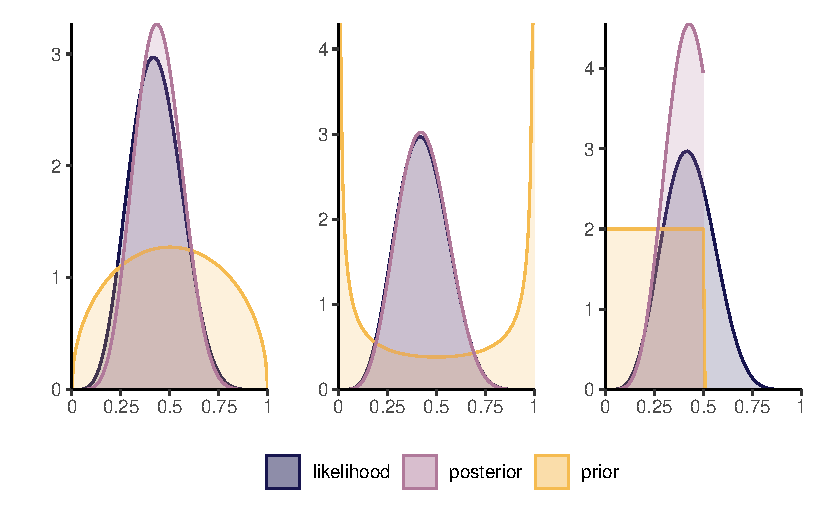
\includegraphics{introduction_files/figure-pdf/fig-betabinom-1.pdf}

}

\caption{\label{fig-betabinom}Binomial likelihood for six successes out
of 14 trials, \(\mathsf{Beta}(3/2, 3/2)\) prior and posterior
distribution from a beta-binomial model. The posterior curve is much
closer to the likelihood than it is to the prior, even with a relatively
small sample size.}

\end{figure}

While a density integrates to 1 over the range of possible outcomes, the
likelihood function does not when we integrate over the range of the
parameters.

We call a prior \emph{proper} if it's integral is finite: the best
example is priors that arise from probability density function. We can
still employ this rule for improper priors: for example, taking
\(\alpha, \beta \to 0\) in the Beta prior leads to a prior proportional
to \(x^{-1}(1-x)^{-1}\), the integral of which diverges on the unit
interval \([0,1]\). However, as long as the number of success and the
number of failures is larger than 1, meaning \(k \geq 1, n-k \geq 1\),
the posterior distribution would be proper, i.e., integrable. To find
the posterior, normalizing constants are also superfluous.

The beta-binomial model is an example of conjugate model, meaning the
posterior distribution is from the same family as the prior.\footnote{This
  is a property of exponential families that will be revisited in the
  next chapter.} While we could calculate analytically the value of the
normalizing constant, we could also in more complicated models use
numerical integration in the event the parameter vector
\(\boldsymbol{\theta}\) is low-dimensional. For a single scalar \(p\) on
the unit interval, numerical integration or Monte Carlo integration
yield nearly identical results.

\begin{Shaded}
\begin{Highlighting}[]
\NormalTok{k }\OtherTok{\textless{}{-}}\NormalTok{ 6L }\CommentTok{\# number of successes }
\NormalTok{n }\OtherTok{\textless{}{-}}\NormalTok{ 14L }\CommentTok{\# number of trials}
\NormalTok{alpha }\OtherTok{\textless{}{-}}\NormalTok{ beta }\OtherTok{\textless{}{-}} \FloatTok{1.5} \CommentTok{\# prior parameters}
\NormalTok{unnormalized\_posterior }\OtherTok{\textless{}{-}} \ControlFlowTok{function}\NormalTok{(p)\{}
\NormalTok{  p}\SpecialCharTok{\^{}}\NormalTok{(k}\SpecialCharTok{+}\NormalTok{alpha}\DecValTok{{-}1}\NormalTok{) }\SpecialCharTok{*}\NormalTok{ (}\DecValTok{1}\SpecialCharTok{{-}}\NormalTok{p)}\SpecialCharTok{\^{}}\NormalTok{(n}\SpecialCharTok{{-}}\NormalTok{k }\SpecialCharTok{+}\NormalTok{ beta }\SpecialCharTok{{-}} \DecValTok{1}\NormalTok{)}
\NormalTok{\}}
\FunctionTok{integrate}\NormalTok{(}\AttributeTok{f =}\NormalTok{ unnormalized\_posterior,}
          \AttributeTok{lower =} \DecValTok{0}\NormalTok{,}
          \AttributeTok{upper =} \DecValTok{1}\NormalTok{)}
\end{Highlighting}
\end{Shaded}

\begin{verbatim}
1.066906e-05 with absolute error < 1e-12
\end{verbatim}

\begin{Shaded}
\begin{Highlighting}[]
\CommentTok{\# Compare with known constant}
\FunctionTok{beta}\NormalTok{(k }\SpecialCharTok{+}\NormalTok{ alpha, n }\SpecialCharTok{{-}}\NormalTok{ k }\SpecialCharTok{+}\NormalTok{ beta)}
\end{Highlighting}
\end{Shaded}

\begin{verbatim}
[1] 1.066906e-05
\end{verbatim}

\begin{Shaded}
\begin{Highlighting}[]
\CommentTok{\# Monte Carlo integration}
\FunctionTok{mean}\NormalTok{(}\FunctionTok{unnormalized\_posterior}\NormalTok{(}\FunctionTok{runif}\NormalTok{(}\FloatTok{1e5}\NormalTok{)))}
\end{Highlighting}
\end{Shaded}

\begin{verbatim}
[1] 1.064055e-05
\end{verbatim}

When \(\boldsymbol{\theta}\) is high-dimensional, the marginal
likelihood is untractable. This is one of the main challenges of
Bayesian statistics and the popularity and applicability has grown
drastically with the development and popularity of numerical algorithms
Gelfand and Smith (\protect\hyperlink{ref-Gelfand.Smith:1990}{1990}).
Markov chain Monte Carlo methods circumvent the calculation of the
denominator by drawing approximate samples from the posterior.

\hypertarget{bayesian-updating}{%
\subsection{Bayesian updating}\label{bayesian-updating}}

Subjective probabilities imply that different people with different
prior beliefs would arrive at different conclusions. However, as more
data are gathered, we can use Bayes theorem to update these prior
beliefs and update the posterior. In most instances, the relative weight
of the prior relative to the likelihood becomes negligible: if we
consider independent data \(\boldsymbol{y}_1, \boldsymbol{y}_n\)
observed sequentially, then \begin{align*}
p(\boldsymbol{\theta} \mid \boldsymbol{y}_1, \ldots, \boldsymbol{y}_k) &\stackrel{\boldsymbol{\theta}}{\propto} p(\boldsymbol{y}_k \mid \boldsymbol{\theta}) p(\boldsymbol{\theta} \mid \boldsymbol{y}_1, \ldots, \boldsymbol{y}_{k-1})
\\ & \stackrel{\boldsymbol{\theta}}{\propto} \prod_{i=1}^k p(\boldsymbol{y}_i \mid \boldsymbol{\theta}) p(\boldsymbol{\theta})
\end{align*} If data are exchangeable, the order in which observations
are collected and the order of the belief updating is irrelevant to the
full posterior
\(p(\boldsymbol{\theta} \mid \boldsymbol{y}_1, \ldots \boldsymbol{y}_n)\).

\bookmarksetup{startatroot}

\hypertarget{priors}{%
\chapter{Priors}\label{priors}}

\bookmarksetup{startatroot}

\hypertarget{references}{%
\chapter*{References}\label{references}}
\addcontentsline{toc}{chapter}{References}

\markboth{References}{References}

\hypertarget{refs}{}
\begin{CSLReferences}{1}{0}
\leavevmode\vadjust pre{\hypertarget{ref-deFinetti:1974}{}}%
Finetti, Bruno de. 1974. \emph{Theory of Probability: A Critical
Introductory Treatment}. Vol. 1. New York: Wiley.

\leavevmode\vadjust pre{\hypertarget{ref-Gelfand.Smith:1990}{}}%
Gelfand, Alan E., and Adrian F. M. Smith. 1990. {``Sampling-Based
Approaches to Calculating Marginal Densities.''} \emph{Journal of the
American Statistical Association} 85 (410): 398--409.
\url{https://doi.org/10.1080/01621459.1990.10476213}.

\leavevmode\vadjust pre{\hypertarget{ref-Geman.Geman:1984}{}}%
Geman, Stuart, and Donald Geman. 1984. {``Stochastic Relaxation, {G}ibbs
Distributions, and the {B}ayesian Restoration of Images.''} \emph{IEEE
Transactions on Pattern Analysis and Machine Intelligence} PAMI-6 (6):
721--41. \url{https://doi.org/10.1109/TPAMI.1984.4767596}.

\leavevmode\vadjust pre{\hypertarget{ref-Jegerlehner:2021}{}}%
Jegerlehner, Sabrina, Franziska Suter-Riniker, Philipp Jent, Pascal
Bittel, and Michael Nagler. 2021. {``Diagnostic Accuracy of a
{SARS-CoV-2} Rapid Antigen Test in Real-Life Clinical Settings.''}
\emph{International Journal of Infectious Diseases} 109 (August):
118--22. \url{https://doi.org/10.1016/j.ijid.2021.07.010}.

\leavevmode\vadjust pre{\hypertarget{ref-owidcoronavirus}{}}%
Mathieu, Edouard, Hannah Ritchie, Lucas Rodés-Guirao, Cameron Appel,
Charlie Giattino, Joe Hasell, Bobbie Macdonald, et al. 2020.
{``Coronavirus Pandemic (COVID-19).''} \emph{Our World in Data}.

\end{CSLReferences}


\backmatter

\end{document}
